\begin{figure}[!h]
\centering
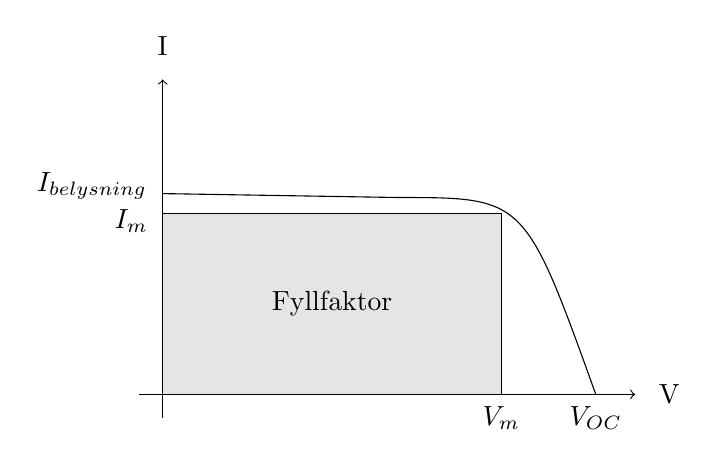
\begin{tikzpicture}

	\draw [->] (-0.3,0) -- (6,0) node [right=5pt]	{V};  % X-akse
	\draw [->] (0,-0.3) -- (0,4) node [above=5pt]	{I}; % Y-akse

	% Faktisk kurve
	\draw [-] (0,2.55) -- (3,2.5);
	\draw [-] (3,2.5) .. controls +(right:1.6cm) .. (5.5,0);
	
	% Fyllfaktor
	\node [draw, rectangle,fill=black!10,minimum height=2.3cm, minimum width=4.3cm] (FF) at (2.15,1.15) {Fyllfaktor};
	
	% Tekst
	\node at (-0.9,2.65) {$I_{belysning}$};
	\node at (-0.4,2.2) {$I_m$};
	\node at (4.3,-0.3) {$V_m$};
	\node at (5.5,-0.3) {$V_{OC}$};
	
	
\end{tikzpicture}

\caption{Str�m-spenningskarakterisitikken for en solcelle}%
\label{fig:fyllfaktor}%
\end{figure}